\chapter{多维随机变量}

在\xref{chap:随机变量及其分布}中,我们仅限于讨论一个随机变量的情形,但在实际问题中,对于某些随机试验的结果,往往需要两个或两个以上的随机变量来描述。正如过去在高等数学中,我们从一元微积分到多元微积分,在本章,我们将把上一章中一维随机变量的概念推广到多维随机变量。

\section{二维随机变量的定义}

\begin{BoxDefinition}[二维随机变量]
    设$E$是一个随机试验,其样本空间$S=\qty{e}$,设
    \begin{Equation}
        X=X(e)\qquad Y=Y(e)
    \end{Equation}
    是定义在$S$上的随机变量,由它们构成一个向量
    \begin{Equation}
        (X,Y)
    \end{Equation}
    称为\uwave{二维随机变量}(Two Dimensional Random Variable)。
\end{BoxDefinition}

二维随机变量$(X,Y)$的性质不仅与$X$与$Y$有关,而且还依赖于这两个随机变量间的相互关系,因此,逐个的研究$X$或$Y$的性质是不够的,还需要将$(X,Y)$作为一个整体来研究。

\subsection{联合分布函数}

二维随机变量也可以类似一维随机变量那样,通过分布函数来研究。

\begin{BoxDefinition}[联合分布函数]*
    设$(X,Y)$是二维随机变量,对于任意实数$x,y$,将二元函数
    \begin{Equation}
        F(x,y)=P\qty{(X\leq x)\cap (Y\leq y)}=P\qty{X\leq x, Y\leq y}
    \end{Equation}
    定义为随机变量$X,Y$的\uwave{联合分布函数}(Joint Distribution Function)。
\end{BoxDefinition}

二维随机变量的分布函数$F(x,y)$继承了很多一维随机变量的分布函数的性质。

\begin{BoxProperty}[二维分布函数的不减性质]
    二维随机变量的分布函数$F(x,y)$是关于$x,y$的不减函数,这就是说
    \begin{itemize}
        \item 对于任意取定的$y$,当$x_2>x_1$时,必有$F(x_2,y)\geq F(x_1,y)$
        \item 对于任意取定的$x$,当$y_2>y_1$时,必有$F(x,y_2)\geq F(x,y_1)$
    \end{itemize}
\end{BoxProperty}

\begin{BoxProperty}[二维分布函数的极限性质]
    二维随机变量的分布函数$F(x,y)$满足以下极限性质
    \begin{Equation}
        \forall y, F(-\infty,y)=0\qquad
        \forall x, F(x,-\infty)=0
    \end{Equation}
    并且
    \begin{Equation}
        F(-\infty,-\infty)=0
    \end{Equation}
    以及
    \begin{Equation}
        F(+\infty,+\infty)=1
    \end{Equation}
\end{BoxProperty}
\xref{ppt:二维分布函数的极限性质}可以这样理解,所谓二维变量的分布函数$F(x,y)$,其实就是指在二维平面上,随机点$(X,Y)$落在一个以$(x,y)$为右上顶点,向左下无限扩展的矩形内的概率。很明显,如果顶点$(x,y)$向左下平移,矩形将越来越“小”,趋于不可能事件,如果顶点$(x,y)$向右上平移,矩形将扩展为全平面,趋于必然事件,这即$F(-\infty,-\infty)=0$和$F(+\infty,+\infty)=1$的直观理解。

\begin{BoxProperty}[二维分布函数的右连续]
    二维随机变量的分布函数$F(x,y)$对$x,y$均是右连续的
    \begin{Equation}
        F(x+0,y)=F(x,y)\qquad
        F(x,y+0)=F(x,y)
    \end{Equation}
\end{BoxProperty}

\begin{BoxProperty}[二维分布函数的非负性]
    二维分布函数$F(x,y)$对于任意$(x_1,y_1)$和$(x_2,y_2)$,$x_1<x_2$,$y_1,y_2$,满足
    \begin{Equation}
        F(x_2,y_2)+F(x_1,y_1)-F(x_2,y_1)-F(x_1,y_2)\geq 0
    \end{Equation}
\end{BoxProperty}

\xref{ppt:二维分布函数的非负性}的表达式在二维平面上绘出了一个以$(x_1,y_1)$和$(x_2,y_2)$为顶点的矩形。

\subsection{二维离散型随机变量}
\begin{BoxDefinition}[二维离散型随机变量]
    设二维随机变量$(X,Y)$,若其全部取值是有限或可列无限多的,记为
    \begin{Equation}
        (x_i,y_i)\quad i,j=1,2,3,\cdots
    \end{Equation}
    则称$(X,Y)$是\uwave{二维离散型随机变量}。

    定义下式为离散型随机变量$X,Y$的联合分布律
    \begin{Equation}
        p_{ij}=P\qty{X=x_i, Y=y_j}\quad i,j=1,2,3,\cdots
    \end{Equation}
    定义下式为离散型随机变量$X,Y$的联合分布函数
    \begin{Equation}
        F(x,y)=\Sum[x_i\leq x]\Sum[y_j\leq y]p_{ij}
    \end{Equation}
    其中和式是对一切满足$x_i\leq x, y_j\leq y$的$i,j$来求和的。
\end{BoxDefinition}

\subsection{二维连续型随机变量}
\begin{BoxDefinition}[二维连续型随机变量]
    设二维随机变量$(X,Y)$,若存在非负函数$f(x,y)$使对于任意$x,y$有
    \begin{Equation}
        F(x,y)=\Int[-\infty][y]\Int[-\infty][x]f(u,v)\dd{u}\dd{v}
    \end{Equation}
    则称$(X,Y)$是\uwave{二维连续性随机变量},其中$f(x,y)$称为$X,Y$的联合概率密度。
\end{BoxDefinition}
对于一维随机变量,其概率密度函数是概率分布的导数
\begin{Equation}
    f(x)=\pdv{F(x)}{x}
\end{Equation}
对于二维随机变量,其概率密度函数是概率分布的二阶混合偏导数
\begin{Equation}
    f(x,y)=\pdv{F(x,y)}{x}{y}
\end{Equation}
类似的,$f(x)\dx$和$f(x,y)\dx\dy$分别表示概率。

\subsection{边缘分布函数}
二维随机变量$(X,Y)$作为一个整体,具有分布函数$F(x,y)$,而$X$和$Y$都是随机变量,理应也可以具有自己的分布函数,那么现在的问题是,如何才能从联合分布函数$F(x,y)$中剥离出随机变量$X$和$Y$自己的分布函数呢?根据\fancyref{def:联合分布函数},$F(x,y)$的定义是
\begin{Equation}
    F(x,y)=P\qty{X\leq x, Y\leq y}
\end{Equation}
而$F_X(x)$和$F_Y(y)$应当是
\begin{Equation}
    F_X(x)=P\qty{X\leq x}\qquad
    F_Y(y)=P\qty{Y\leq y}
\end{Equation}
这里$F_X(x),F_Y(y)$中,对$Y$和$X$是无要求的,换言之
\begin{Equation}
    F_X(x)=P\qty{X\leq x, Y<\infty}\qquad
    F_Y(y)=P\qty{X<\infty,Y\leq y}
\end{Equation}
这就是边缘分布函数的来历,我们正式的定义如下。
\begin{BoxDefinition}[边缘分布函数]
    设$(X,Y)$是二维随机变量,对于任意实数,将
    \begin{Equation}
        F_X(x)=P\qty{X\leq x, Y<\infty}\qquad
        F_Y(y)=P\qty{X<\infty,Y\leq y}
    \end{Equation}
    定义为随机变量$X,Y$的\uwave{边缘分布函数}(Marginal Distribution Function)。
\end{BoxDefinition}

通过\xref{fig:联合分布与边缘分布},我们可以直观的看到联合分布与边缘分布的差异
\begin{Figure}[联合分布与边缘分布]
    \begin{FigureSub}[联合分布$F(x,y)$;联合分布]
        \includegraphics[width=4.2cm]{build/Chapter03A_01.fig.pdf}
    \end{FigureSub}
    \hspace{0.5cm}
    \begin{FigureSub}[边缘分布$F_X(x)$;边缘分布X]
        \includegraphics[width=4.2cm]{build/Chapter03A_02.fig.pdf}
    \end{FigureSub}
    \hspace{0.5cm}
    \begin{FigureSub}[边缘分布$F_Y(y)$;边缘分布Y]
        \includegraphics[width=4.2cm]{build/Chapter03A_03.fig.pdf}
    \end{FigureSub}
\end{Figure}
基于边缘分布函数,我们可以分别定义离散型的边缘分布律和连续型的边缘概率密度。

\begin{BoxDefinition}[边缘分布律]
    对于离散型二维随机变量$(X,Y)$,定义\uwave{边缘分布律}
    \begin{Gather}[8pt]
        p_{i \cdot}=P\qty{X=x_i}=\Sum[j=1][\infty]p_{ij}\qquad i=1,2,\cdots\\
        p_{\cdot j}=P\qty{Y=y_j}=\Sum[i=1][\infty]p_{ij}\qquad j=1,2,\cdots
    \end{Gather}
\end{BoxDefinition}

\begin{BoxDefinition}[边缘概率密度]
    对于连续型二维随机变量$(X,Y)$,定义\uwave{边缘概率密度}
    \begin{Gather}[8pt]
        f_X(x)=\Int[-\infty][\infty]f(x,y)\dy\\
        f_Y(y)=\Int[-\infty][\infty]f(x,y)\dx
    \end{Gather}
\end{BoxDefinition}

简而言之,研究某个随机变量的边缘分布律或边缘概率密度,就是在联合分布律或联合概率密度中,令该变量固定,令另外一个变量取所有值,将所有结果进行求和或积分即可。

离散型二维随机变量的分布律常以表格的形式呈现,如\xref{tab:离散型二维随机变量的分布律}
\begin{Table}[离散型二维随机变量的分布律]{|c|cccc|c|}
<>
$p_{ij}$&$j=1$&$j=2$&$\cdots$&$j=J$&$p_{i\cdot}$\\ \hlinelig
$i=1$&$p_{11}$&$p_{12}$&$\cdots$&$p_{1B}$&$p_{1\cdot}$\\ 
$i=2$&$p_{21}$&$p_{12}$&$\cdots$&$p_{2B}$&$p_{2\cdot}$\\ 
$\vdots$&$\vdots$&$\vdots$&$\ddots$&$\vdots$&$\vdots$\\
$i=A$&$p_{A1}$&$p_{A2}$&$\cdots$&$p_{AB}$&$p_{A\cdot}$\\ \hlinelig
$p_{\cdot j}$&$p_{\cdot 1}$&$p_{\cdot 2}$&$\cdots$&$p_{\cdot B}$&/\\
\end{Table}
注意到,联合分布位于表格中间,边缘分布则位于表格边缘,这就是边缘分布的得名由来。 

\subsection{二维正态分布}
我们可以将\fancyref{def:正态分布}推广到二维情况中
\begin{BoxDefinition}[二维正态分布]*
    若二维连续性随机变量$(X,Y)$具有概率密度
    \begin{Equation}
        f(x,y)=\frac{1}{2\pi\sigma_1\sigma_2\sqrt{1-\rho^2}}\exp\qty{
            \frac{-1}{2(1-\rho^2)}
            \qty[
            \frac{(x-\mu_1)^2}{\sigma_1^2}
            \hspace{-0.1em}-\hspace{-0.1em}
            2\rho\frac{(x\hspace{-0.1em}-\hspace{-0.1em}\mu_1)(x\hspace{-0.1em}-\hspace{-0.1em}\mu_2)}{\sigma_1\sigma_2}
            \hspace{-0.1em}+\hspace{-0.1em}
            \frac{(y-\mu_2)^2}{\sigma_2^2}]
        }
    \end{Equation}
    则称$(X,Y)$服从参数为$\mu_1,\mu_2,\sigma_1,\sigma_2,\rho$的\uwave{二维正态分布},记为
    \begin{Equation}
        (X,Y)\sim N(\mu_1,\mu_2,\sigma_1,\sigma_2)
    \end{Equation}
\end{BoxDefinition}
\xref{fig:二维正态分布}绘制了典型的二维正态分布的图像,取参数$\mu_1=\mu_2=0$,$\sigma_1=\sigma_2=0.4$,$\rho=0$
\begin{Figure}[二维正态分布]
    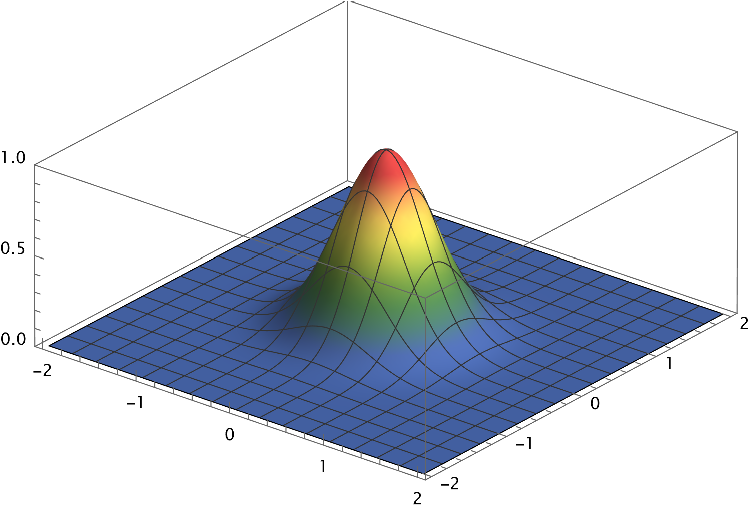
\includegraphics[scale=0.75]{Mathematica/output/Gauss2D44.pdf}
    \hspace{0.2cm}
    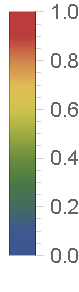
\includegraphics[scale=1.0]{Mathematica/output/Gauss2DColorbar.pdf}
\end{Figure}
二维正态分布中的参数$\mu_1,\mu_2,\sigma_1,\sigma_2,\rho$的意义与一维情形相类似,$\mu_1,\mu_2$代表了$x,y$方向上的中心(均值),$\sigma_1,\sigma_2$代表了$x,y$方向上的集中程度(方差),$\rho$则是二维正态分布中的一个新参数,它代表了$x,y$方向上的某种联系(相关系数),\xref{tab:二维正态分布的参数}以等值线表现了参数的意义,形象的说,参数$\rho$会使得图形在$45^{\circ}$方向上被拉长,同时,参数$\rho$越大图形的中心也会更高。

\begin{Table}[二维正态分布的参数]{|c|c|c|c|c|}
<>
\xcell<c>[2ex][0ex]{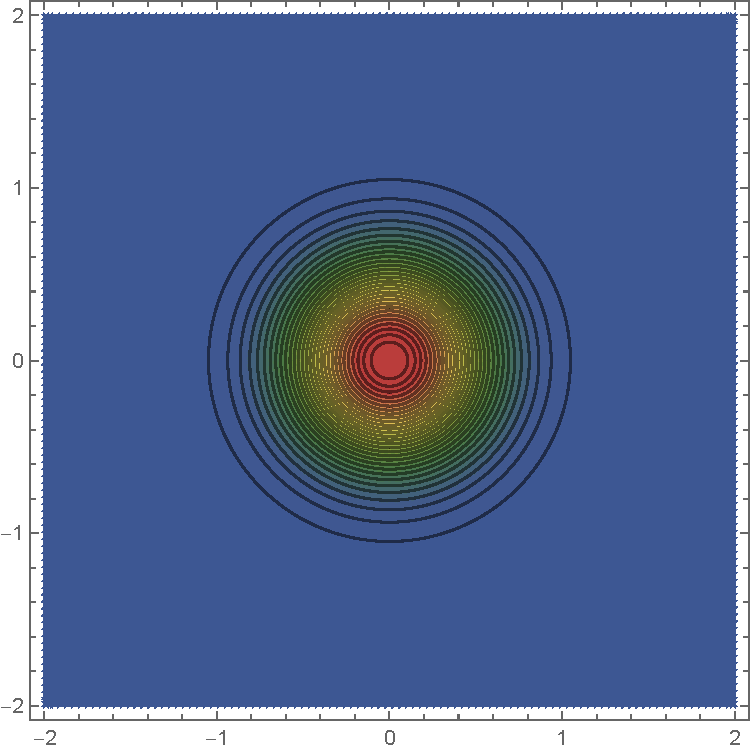
\includegraphics[width=3cm]{Mathematica/output/Gauss44.pdf}}&
\xcell<c>[2ex][0ex]{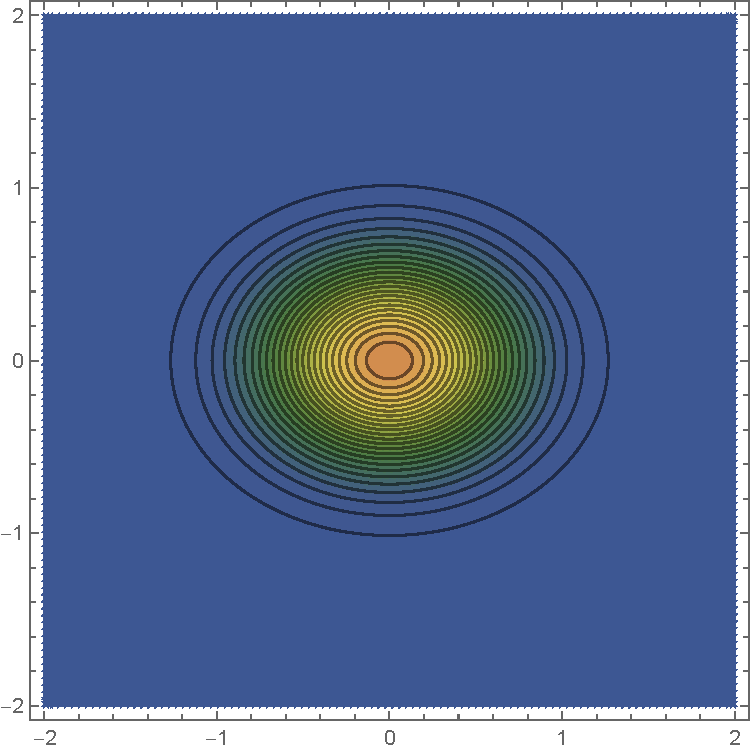
\includegraphics[width=3cm]{Mathematica/output/Gauss54.pdf}}&
\xcell<c>[2ex][0ex]{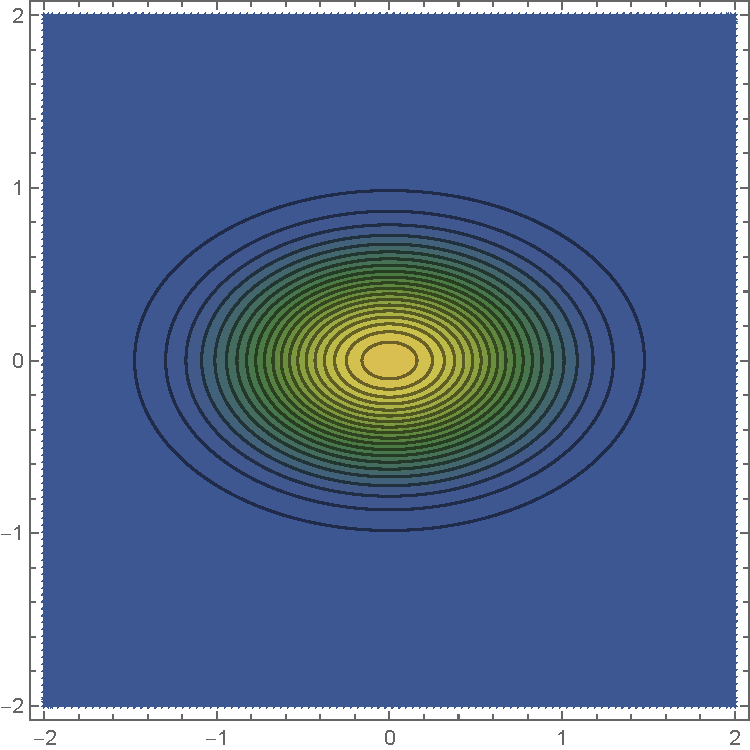
\includegraphics[width=3cm]{Mathematica/output/Gauss64.pdf}}&
\xcell<c>[2ex][0ex]{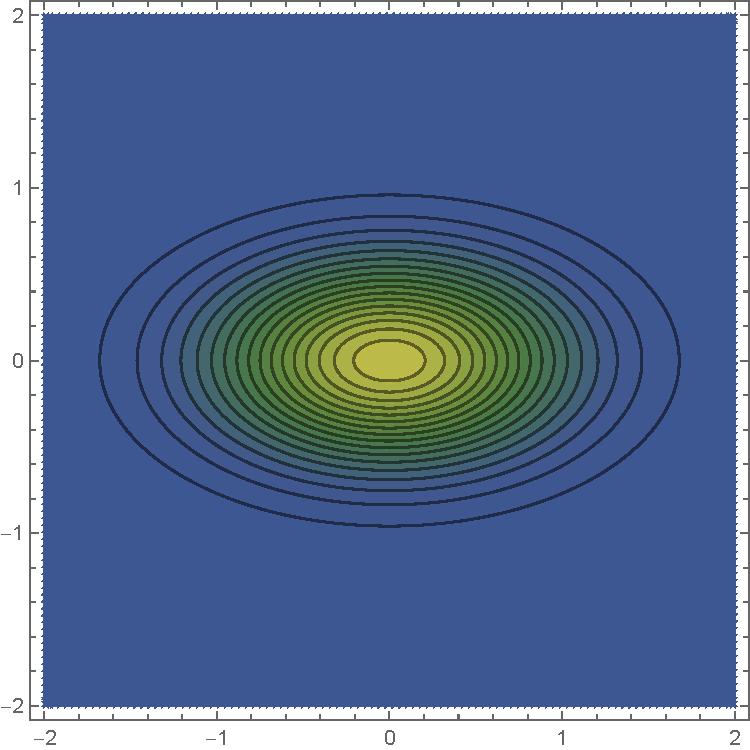
\includegraphics[width=3cm]{Mathematica/output/Gauss74.pdf}}\\
$\sigma_1=0.4,~\sigma_2=0.4$&
$\sigma_1=0.5,~\sigma_2=0.4$&
$\sigma_1=0.6,~\sigma_2=0.4$&
$\sigma_1=0.7,~\sigma_2=0.4$\\
$\rho=0.00$&
$\rho=0.00$&
$\rho=0.00$&
$\rho=0.00$\\
\hlinemid
\xcell<c>[2ex][0ex]{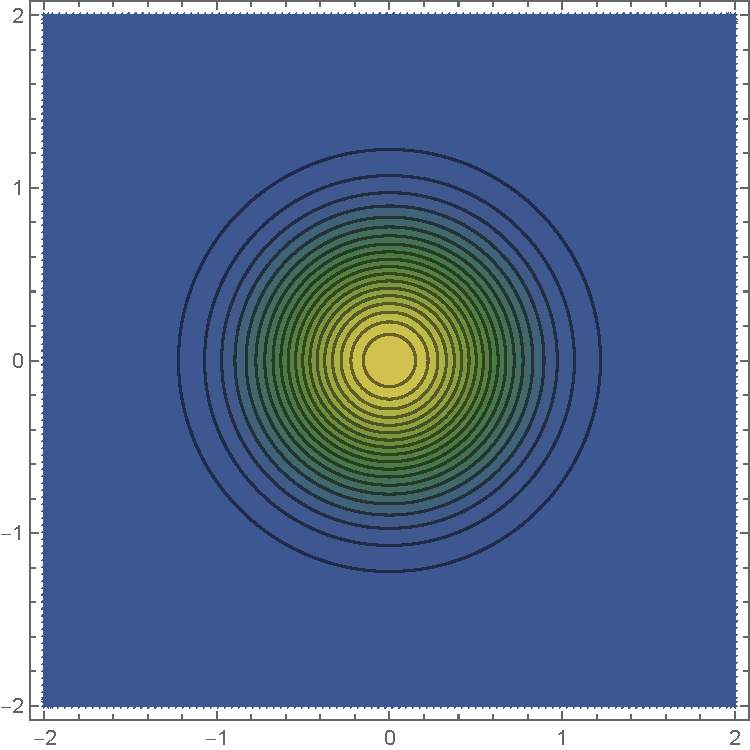
\includegraphics[width=3cm]{Mathematica/output/Gauss55_0.pdf}}&
\xcell<c>[2ex][0ex]{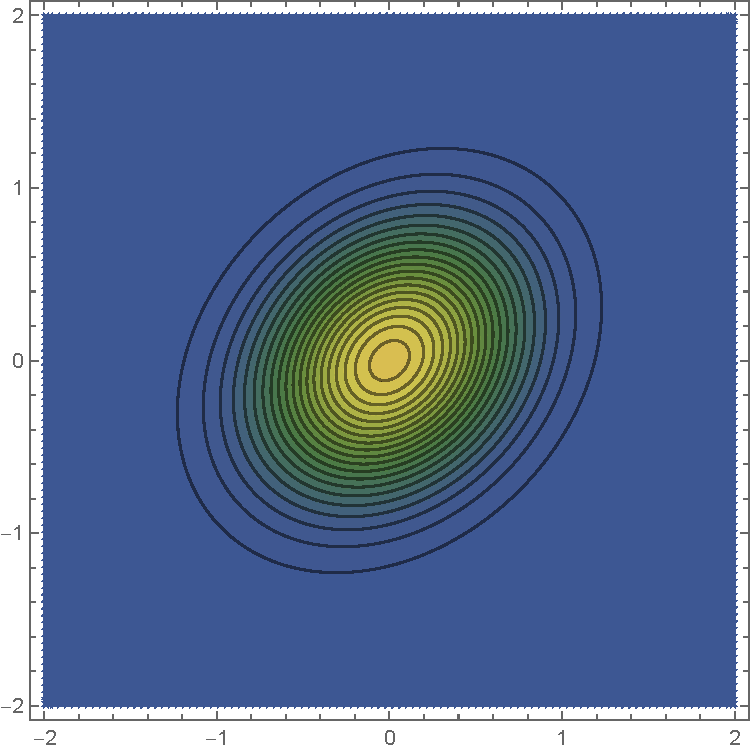
\includegraphics[width=3cm]{Mathematica/output/Gauss55_25.pdf}}&
\xcell<c>[2ex][0ex]{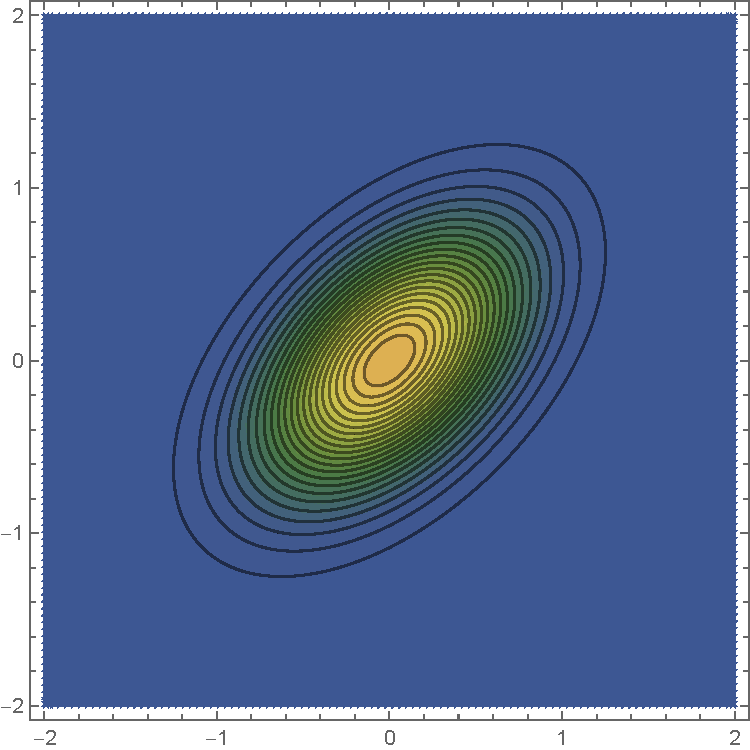
\includegraphics[width=3cm]{Mathematica/output/Gauss55_50.pdf}}&
\xcell<c>[2ex][0ex]{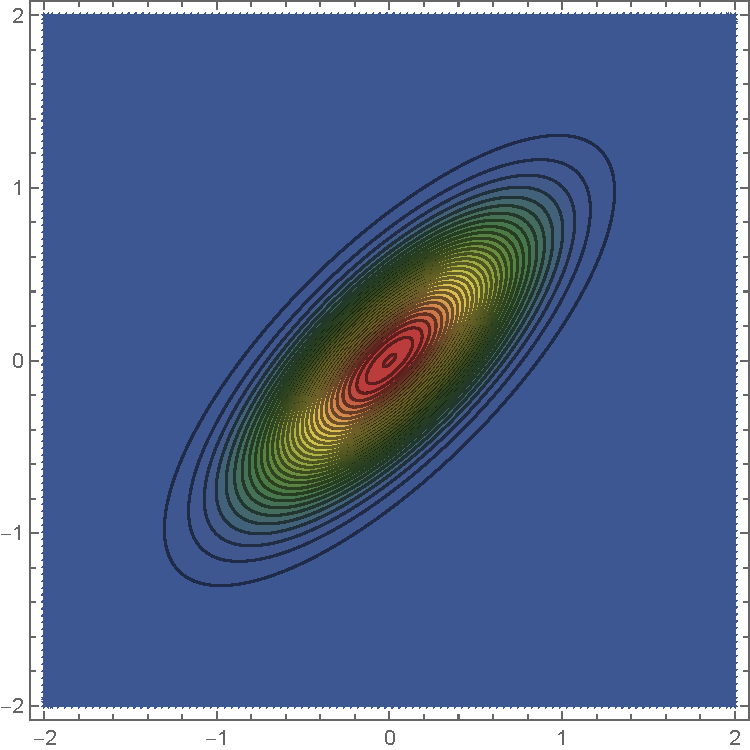
\includegraphics[width=3cm]{Mathematica/output/Gauss55_75.pdf}}\\
$\sigma_1=0.5,~\sigma_2=0.5$&
$\sigma_1=0.5,~\sigma_2=0.5$&
$\sigma_1=0.5,~\sigma_2=0.5$&
$\sigma_1=0.5,~\sigma_2=0.5$\\
$\rho=0.00$&
$\rho=0.25$&
$\rho=0.50$&
$\rho=0.75$\\
\end{Table}

\begin{BoxFormula}[二维正态分布的边缘分布]
    二维正态分布在$x$方向的边缘分布为
    \begin{Equation}
        f_X(x)=\frac{1}{\sqrt{2\pi}\sigma_1}\exp[-\frac{(x-\mu_1)^2}{2\sigma_1^2}]
    \end{Equation}
    二维正态分布在$y$方向的边缘分布为
    \begin{Equation}
        f_Y(y)=\frac{1}{\sqrt{2\pi}\sigma_2}\exp[-\frac{(y-\mu_2)^2}{2\sigma_2^2}]
    \end{Equation}
\end{BoxFormula}

\begin{Proof}
    根据\fancyref{def:二维正态分布}
    \begin{Equation}&[1]
        f(x,y)=\frac{1}{2\pi\sigma_1\sigma_2\sqrt{1-\rho^2}}\exp\qty{
            \frac{-1}{2(1-\rho^2)}
            \qty[
            \frac{(x-\mu_1)^2}{\sigma_1^2}
            -
            2\rho\frac{(x-\mu_1)(x-\mu_2)}{\sigma_1\sigma_2}
            +
            \frac{(y-\mu_2)^2}{\sigma_2^2}]
        }
    \end{Equation}
    根据\fancyref{def:边缘概率密度},先求$x$方向的边缘概率密度
    \begin{Equation}&[2]
        f_X(x)=\Int[-\infty][\infty]f(x,y)\dd{y}
    \end{Equation}
    我们注意到
    \begin{Equation}&[3]
        \frac{(y-\mu_2)^2}{\sigma_2^2}-2\rho\frac{(x-\mu_1)(y-\mu_2)}{\sigma_1\sigma_2}=
        \frac{(y-\mu_2)^2}{\sigma_2^2}-2\rho\frac{(x-\mu_1)(y-\mu_2)}{\sigma_1\sigma_2}+\rho^2\frac{(x-\mu_1)^2}{\sigma_1^2}-\rho^2\frac{(x-\mu_1)^2}{\sigma_1^2}
    \end{Equation}
    即
    \begin{Equation}&[4]
        \qquad\qquad
        \frac{(y-\mu_2)^2}{\sigma_2^2}-2\rho\frac{(x-\mu_1)(y-\mu_2)}{\sigma_1\sigma_2}=
        \qty(\frac{y-\mu_2}{\sigma_2}-\rho\frac{x-\mu_1}{\sigma_1})^2-\rho^2\frac{(x-\mu_1)^2}{\sigma_1^2}
        \qquad\qquad
    \end{Equation}
    将\xrefpeq{4}代入\xrefpeq{1}
    \begin{Equation}&[5]
        \qquad
        f(x,y)=\frac{1}{2\pi\sigma_1\sigma_2\sqrt{1-\rho^2}}\exp\qty{
            -\frac{(x-\mu_1)^2}{2\sigma_1^2}+
            \frac{-1}{2(1-\rho^2)}
            \qty(\frac{y-\mu_2}{\sigma_2}-\rho\frac{x-\mu_1}{\sigma_1})^2
        }
        \qquad
    \end{Equation}
    试将\xrefpeq{5}按照\xrefpeq{2}积分
    \begin{Equation}&[6]
        f_X(x)=\frac{1}{2\pi\sigma_1\sigma_2\sqrt{1-\rho^2}}
        \exp[-\frac{(x-\mu_1)^2}{2\sigma_1^2}]
        \Int[-\infty][\infty]
        \exp[
            \frac{-1}{2(1-\rho^2)}
            \qty(\frac{y-\mu_2}{\sigma_2}-\rho\frac{x-\mu_1}{\sigma_1})^2
            ]\dd{y}
    \end{Equation}
    作变量代换
    \begin{Equation}&[7]
        t=\frac{1}{\sqrt{1-\rho^2}}
        \qty(\frac{y-\mu_2}{\sigma_2}-\rho\frac{x-\mu_1}{\sigma_1})
    \end{Equation}
    注意到
    \begin{Equation}&[8]
        \dd{y}=\frac{\sqrt{1-\rho^2}}{\sigma_2}\dd{t}
    \end{Equation}
    将\xrefpeq{7}和\xrefpeq{8}代入\xrefpeq{6}
    \begin{Equation}&[9]
        f_X(x)=\frac{1}{2\pi\sigma_1}\exp[-\frac{(x-\mu_1)^2}{2\sigma_1^2}]\Int[-\infty][\infty]\exp(-t^2/2)\dd{t}
    \end{Equation}
    这个积分我们很熟悉,结果是$\sqrt{2\pi}$,故
    \begin{Equation}&[10]
        f_X(x)=\frac{1}{\sqrt{2\pi}\sigma_1}\exp[-\frac{(x-\mu_1)^2}{2\sigma_1^2}]
    \end{Equation}
    完全类似的
    \begin{Equation}&[11]
        f_Y(y)=\frac{1}{\sqrt{2\pi}\sigma_2}\exp[-\frac{(y-\mu_2)^2}{2\sigma_2^2}]
    \end{Equation}
    至此,我们就得到了二维高斯分布的两个边缘函数。
\end{Proof}

在\xref{fml:二维正态分布的边缘分布}中,我们注意到,二维正态分布的两个边缘分布$f_X(x),f_Y(y)$均与参数$\rho$无关,换言之,对于给定的$\mu_1,\mu_2,\sigma_1,\sigma_2$,无论$\rho$的取值如何,边缘分布都是一样的。这一事实告诉我们,由联合分布可以确定边缘分布,但反过来,由边缘分布是无法唯一确定联合分布的。

